\documentclass{article}
\usepackage{xcolor}
\newcommand{\myhighlight}[1]{\textcolor{blue}{#1}}

% The draft follows the supplied NeurIPS-style template when the local style
% file exists, and falls back to a standard preprint layout in this workspace.
\IfFileExists{neurips_2026.sty}{%
  \usepackage{neurips_2026}
}{%
  \usepackage[margin=1in]{geometry}
  \usepackage[numbers,sort&compress]{natbib}

}

\usepackage[utf8]{inputenc}
\usepackage[T1]{fontenc}
\usepackage{hyperref}
\usepackage{url}
\usepackage{booktabs}
\usepackage{amsfonts}
\usepackage{amsmath}
\usepackage{amssymb}
\usepackage{nicefrac}
\usepackage{microtype}
\usepackage{xcolor}
\usepackage{enumitem}
\usepackage{tabularx}
\usepackage{array}
\usepackage{graphicx}
\usepackage{tikz}
\usetikzlibrary{arrows.meta, positioning, patterns}

\usepackage{mathtools}
\usepackage{amsthm}
\theoremstyle{plain}
% \newtheorem{findings}{Findings}
\newtheorem{desideratum}{Desideratum}
\renewcommand{\thedesideratum}{\Roman{desideratum}}



\hypersetup{
  colorlinks=true,
  linkcolor=blue,
  citecolor=blue,
  urlcolor=blue
}

\title{\textcolor{blue}{TokenShare: Sharing Tokenized Intelligent Capacity for Verifiable Useful Work}}
\author{Hongzhan Tu \and Zhizhou Wang}

\begin{document}

\maketitle

\begin{abstract}
{\color{blue}
Large useful tasks increasingly require more than a single model invocation. They consume model tokens, tool calls, local compute, formal checkers, human attention, retries, and verification effort. Individually, these resources are fragmented across people, machines, organizations, and agents; collectively, they form a latent pool of intelligent capacity. This paper proposes \emph{TokenShare}: the concept of turning fragmented tokenized capacity into verifiable, mergeable, and accountable contributions to a larger task.

The distributed system in this paper is an instrument for making that concept concrete. It represents a task as a recursively expandable task DAG, assigns bounded units through leases and attempts, persists submissions and artifacts, verifies outputs through task plugins, merges accepted child results, and records contribution accounting in an append-only event ledger. We instantiate TokenShare with two real proof-of-concept domains: integer factorization with deterministic range verification and Lean formal-proof production with a fixed local Lean/lake checker environment. We also evaluate an experiment-scoped AI API executor that records raw model output, parsed output, parse failure, usage, cost, latency, and provider provenance. Across 17 default experiment runs, TokenShare exercises end-to-end useful-work sharing, failure isolation, mechanism ablation, and cross-domain generality, producing 1215 events and 510 artifacts. The evidence supports the central claim: shared tokenized capacity becomes useful only when the system can decompose work, verify contributions, merge accepted evidence, and replay why each contribution counted.
}
\end{abstract}

\section{Introduction}

{\color{blue}
The simplest intuition behind modern AI work is that more attempts can buy more capability. A model may solve a problem after additional tokens, a tool call may expose missing evidence, a proof checker may reject a plausible answer, and a human reviewer may repair an ambiguous output. These attempts are not free. They consume tokenized units of intelligent capacity: model tokens, API calls, local compute, formal-checker time, domain expertise, and human attention.

Many useful tasks need more capacity than one user, model session, machine, or organization can conveniently spend. Scientific computation, formal reasoning, benchmark construction, data transformation, annotation, and public-good knowledge work all require decomposition, bounded execution, verification, repair, and integration. At the same time, useful capacity is widely scattered: idle local machines, unused API credits, personal agents, laboratory servers, tool environments, and human reviewers often hold small but meaningful pieces of the required work.

TokenShare is the proposal that those fragmented units can be shared as contributions to a common useful task. The essential idea is not merely parallel execution. A shared token must become a contribution: it must be attached to a task unit, bounded by an execution request, preserved as evidence, checked by a task-specific verifier, selected into canonical state, merged with other accepted evidence, and recorded so that later participants can audit why it mattered. The distributed-system machinery in this paper exists to enforce that conversion from spent capacity to accepted contribution.
}

This paper makes three main \textbf{contributions}:

\begin{itemize}
\item \textcolor{blue}{We formulate TokenShare as a shared-capacity concept: fragmented model tokens, tool calls, compute, checker time, and human attention can be converted into verifiable contributions to decomposable useful work.}
 \item \textcolor{blue}{We show how a distributed protocol can operationalize this concept through task DAGs, leases, artifact-backed submissions, plugin-owned verification, canonical selection, merge, contribution accounting, and replayable evidence.}
\item  \textcolor{blue}{We evaluate the concept with real factorization and Lean proof plugins, failure injection, mechanism ablation, cross-plugin generality, and a real AI API executor profile, clarifying what each experiment demonstrates about useful token sharing.}
\end{itemize}






\section{\textcolor{blue}{Motivation Towards Shared Token Economics}}


\subsection{Background}

\textbf{\textcolor{blue}{Tokens as Units of Intelligent Capacity}}~
{\color{blue}
In TokenShare, a ``token'' is broader than a language-model token. It is any bounded unit of intelligent capacity that can be spent toward a task: a model call, a tool invocation, a local computation slice, a checker run, a repair attempt, or a unit of human review. The point of sharing tokens is not to pool raw expenditure for its own sake, but to make small resource contributions composable into a larger verified output.
}

\textbf{\textcolor{blue}{The Price of Useful Sharing}}~
{\color{blue}
Sharing capacity is easy when correctness does not matter; it is hard when the final artifact must be trusted. A useful shared contribution must answer four questions: what resource was spent, what task unit it addressed, what evidence it produced, and why that evidence was accepted or rejected. TokenShare treats those questions as first-class protocol data rather than after-the-fact narration.
}


\subsection{Motivations}

{\color{blue}
The motivating question is therefore: \emph{Can a community share tokenized intelligent capacity in a way that produces useful work rather than unstructured effort?}

TokenShare answers by separating the concept from the tool that realizes it. Conceptually, TokenShare is a contribution economy for useful intelligent work: shared resources should become accepted contributions only after they are bounded, evidenced, verified, and mergeable. Operationally, the prototype uses a local distributed-systems design to enforce those properties. The protocol core maintains task units, dependency edges, leases, attempts, artifact references, verification reports, canonical output bindings, expansion decisions, merge records, contribution records, and accounting records.

A task plugin defines what counts as a valid contribution for a domain; an executor merely spends capacity and returns evidence. This boundary is central to TokenShare. A model-backed contributor may spend tokens, but raw text alone is evidence rather than contribution. A range worker may spend compute, but a false factor claim is rejected expenditure rather than useful work. A Lean proof attempt may spend checker time, but only a checker-backed proof artifact can count. TokenShare is the bridge between resource expenditure and accepted contribution.
}

\section{The Design Philosophy}
\subsection{Problem Formulation}

{\color{blue}
We consider a useful root task $T$ and a population of contributors who can spend heterogeneous tokenized resources:
\[
\mathcal{K}=\{k_1,k_2,\ldots,k_m\},
\]
where a token $k_i$ may be a model call, local computation interval, checker invocation, tool call, or human review action. TokenShare is concerned with when a spent token becomes a contribution. We model an accepted contribution as
\[
c=(u, k_i, a, e, v, m),
\]
where $u$ is the task unit, $a$ is the execution attempt, $e$ is the produced evidence artifact, $v$ is the verification result, and $m$ is the merge or accounting relation that explains how the contribution affects the larger task.

The implementation realizes this concept as a protocol instance
\[
\mathcal{P}_T=(G_T,\mathcal{A}_T,\mathcal{E}_T,\mathcal{R}_T),
\]
where $G_T$ is the task DAG, $\mathcal{A}_T$ is the content-addressed evidence set, $\mathcal{E}_T$ is the append-only event log, and $\mathcal{R}_T$ freezes the plugin and executor descriptors used by the run. The distributed system is therefore not the definition of TokenShare; it is the evidence machine that makes shared contributions assignable, checkable, mergeable, and replayable.

Recursive decomposition controls the granularity at which tokens can be shared. A plugin-owned split strategy may transform an already verified canonical output bundle into
\[
\mathrm{Split}_p(u,\hat{Y}_u)\rightarrow(\Delta G, \mathrm{MergePlan}),
\]
where $\Delta G$ contains child units and dependencies, and the merge plan records the required child output slots. This is the key design move: TokenShare can invite more capacity into the system only when the resulting units have explicit inputs, expected outputs, verification rules, and merge obligations.
}



\subsection{Desiderata of TokenShare Protocol}


\begin{desideratum}
\textbf{Decomposability:}~ A TokenShare task should be expressible as a structured task tree or directed acyclic graph whose executable units have clear inputs, outputs, dependencies, and merge relations.
\end{desideratum}

{\color{blue}
A TokenShare task must be decomposable into units small enough for shared contributors to execute, but structured enough for the result to rejoin the parent task. Decomposition is therefore not a free-form plan emitted by an executor; it is a versioned plugin decision recorded through a structured proposal and an expansion event batch. In the factorization plugin, decomposition partitions a candidate divisor domain into bounded range units. In the Lean plugin, decomposition is produced by a deterministic Lean-side helper that emits a split certificate and a merge skeleton. In both cases, decomposition creates shareable contribution opportunities without giving contributors authority over the task graph.
}


\begin{desideratum}
\textbf{Local Verifiability:}~ \textcolor{blue}{Each executable subtask should include an explicit verifier that can check whether its submitted output is valid before that output is accepted, merged, or counted as eligible contribution evidence.}
\end{desideratum}

{\color{blue}
Each candidate output must be verifiable before it becomes a contribution. TokenShare separates parsing, structural checks, domain verification, and canonical selection. For factorization, the plugin verifier rechecks whether a claimed factor divides the target and whether a no-factor range claim is consistent with its bounded domain. For Lean proof production, the validator accepts only checker reports backed by a fixed local Lean/lake environment, generated source, stdout/stderr logs, proof artifacts, and an environment reference. A raw model response or executor submission is therefore evidence, not authority.
}


\begin{desideratum}
\textbf{Extendability:}~ The protocol should provide a reusable coordination skeleton while allowing each task family to plug in task-specific schemas, verifiers, merge rules, cost models, and contributor requirements.
\end{desideratum}

{\color{blue}
The concept should survive beyond a single task family. TokenShare implements extendability through frozen plugin descriptors and executor descriptors. A plugin supplies task types, schemas, parser policy, split strategy, validator policy, and merge policy. An executor supplies a transport or local execution boundary and returns artifacts. This makes the same contribution lifecycle coordinate arithmetic range search and Lean proof checking while keeping divisibility rules and proof-checking rules outside the shared protocol.
}


\begin{desideratum}
\textbf{Scalability:}~ As more tokens, agents, workers, or computational resources become available, the protocol should convert that additional capacity into faster completion, higher quality, broader verification, or stronger fault tolerance.
\end{desideratum}

{\color{blue}
The relevant scaling unit is not only the number of workers, but the amount of independently checkable evidence the system can admit without corrupting accepted state. TokenShare therefore scales through smaller typed artifacts, explicit lease and attempt records, deterministic merge gates, and replayable event batches. Additional tokenized capacity is useful only when its output can be parsed, verified, linked to an expected slot, and merged under a recorded policy.
}


\begin{desideratum}
\textbf{Autonomy:}~ \textcolor{blue}{The protocol should advance tasks through assignment, execution, validation, verification, merging, timeout recovery, reassignment, and contribution accounting according to predefined rules with minimal continuous manual coordination.}
\end{desideratum}

{\color{blue}
The protocol should advance routine lifecycle transitions from recorded facts rather than conversational memory. A request produces a submission; a submission produces a verification report; verified candidates may compete for a single canonical output bundle; canonical outputs may trigger completion or expansion; merge records and expected-output resolution produce parent completion; eligible canonical contributions enter an accounting batch. The autonomy claim is therefore conceptual and operational: shared tokens can be converted into work units without constant manual coordination, and the system can later explain why a task progressed, blocked, or rejected an output.
}



\section{The TokenShare Protocol}

{\color{blue}
The TokenShare protocol is the mechanism that turns the concept of shared tokenized capacity into executable work. Its purpose is to decide when resource expenditure becomes accepted contribution. The implementation has three boundaries: protocol objects and state transitions, task plugins, and executors. Protocol objects define the reusable contribution lifecycle; plugins define task semantics; executors spend resources and produce submissions under a request contract. The event ledger and artifact store connect the three layers by making every authority-bearing fact persistent.
}

\subsection{Overall Picture}

{\color{blue}
Figure~\ref{fig:tokenshare-overall} shows how the concept is implemented. A root task enters the system as a typed request for shared work. The protocol engine turns that request into shareable task units, records registry snapshots, schedules ready units through leases, records execution requests and submissions, invokes verification and canonical selection, accepts plugin-owned expansion proposals, resolves merge tasks, and records contribution accounting. SQLite is a materialized index over the append-only event ledger rather than the source of authority.
}

\begin{figure}[htbp]
\centering
\resizebox{\linewidth}{!}{
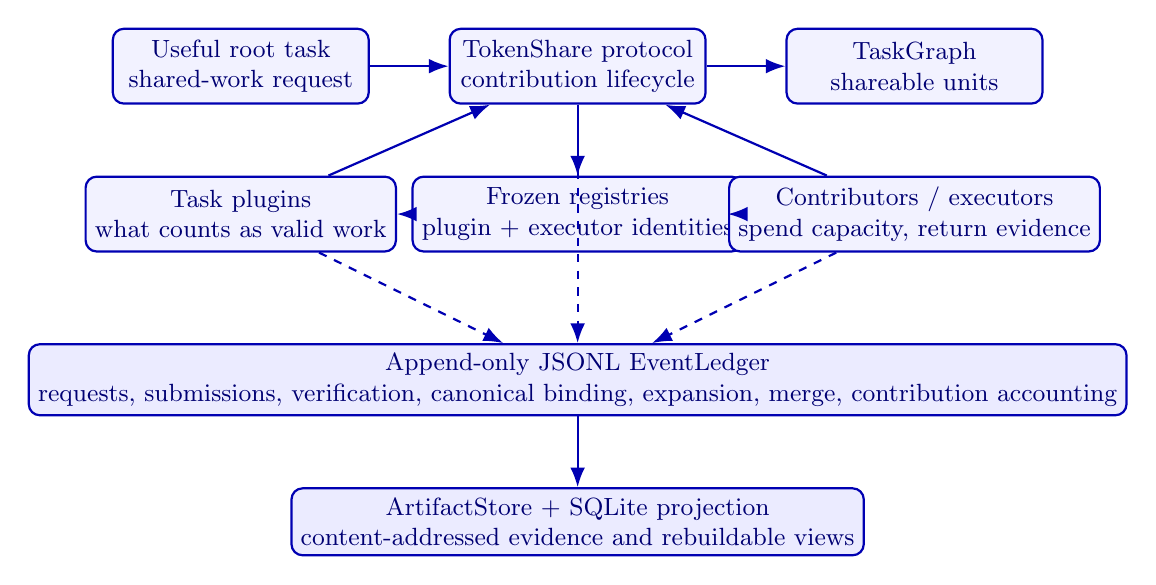
\begin{tikzpicture}[
    node distance=0.9cm and 1.0cm,
    box/.style={
        rectangle,
        rounded corners,
        draw=blue!70!black,
        fill=blue!5,
        thick,
        align=center,
        minimum width=3.25cm,
        minimum height=0.95cm,
        font=\small,
        text=blue!45!black
    },
    wide/.style={
        rectangle,
        rounded corners,
        draw=blue!70!black,
        fill=blue!8,
        thick,
        align=center,
        minimum width=7.1cm,
        minimum height=0.85cm,
        font=\small,
        text=blue!45!black
    },
    arrow/.style={-{Latex[length=2.5mm]}, thick, draw=blue!70!black},
    dashedarrow/.style={-{Latex[length=2.5mm]}, thick, dashed, draw=blue!70!black}
]

\node[box] (input) {Useful root task\\shared-work request};
\node[box, right=of input] (engine) {TokenShare protocol\\contribution lifecycle};
\node[box, right=of engine] (graph) {TaskGraph\\shareable units};

\node[box, below=of engine] (registry) {Frozen registries\\plugin + executor identities};
\node[box, below=of input] (plugins) {Task plugins\\what counts as valid work};
\node[box, below=of graph] (executors) {Contributors / executors\\spend capacity, return evidence};

\node[wide, below=1.15cm of registry] (ledger) {Append-only JSONL EventLedger\\requests, submissions, verification, canonical binding, expansion, merge, contribution accounting};
\node[wide, below=of ledger] (store) {ArtifactStore + SQLite projection\\content-addressed evidence and rebuildable views};

\draw[arrow] (input) -- (engine);
\draw[arrow] (engine) -- (graph);
\draw[arrow] (engine) -- (registry);
\draw[arrow] (registry) -- (plugins);
\draw[arrow] (registry) -- (executors);
\draw[arrow] (plugins) -- (engine);
\draw[arrow] (executors) -- (engine);
\draw[dashedarrow] (engine) -- (ledger);
\draw[dashedarrow] (plugins) -- (ledger);
\draw[dashedarrow] (executors) -- (ledger);
\draw[arrow] (ledger) -- (store);

\end{tikzpicture}
}
\caption{\textcolor{blue}{TokenShare as a concept implemented by a distributed protocol. Contributors and executors spend tokenized capacity; plugins decide what counts as valid work in a domain; the protocol records the contribution lifecycle that makes accepted work shareable, mergeable, and auditable.}}
\label{fig:tokenshare-overall}
\end{figure}

\subsection{Task Registration, Decomposition, Assignment, and Commitment}

\subsubsection{Task Registration}

{\color{blue}
A registered task is a typed protocol object rather than an informal request. The root \texttt{TaskUnit} stores a \texttt{TaskSpec}, plugin identity, required outputs, dependency state, and artifact references. The input body is persisted through a content-addressed artifact reference, and task creation is recorded as an event. This gives later verification and replay a stable object identity:
\[
\mathrm{Root}(T)=
(\mathrm{task\_id},\mathrm{unit\_id},\mathrm{plugin\_id},\mathrm{input\_ref},\mathrm{required\_outputs}).
\]
}

\subsubsection{Recursive Task Decomposition}

{\color{blue}
TokenShare expands only from accepted evidence. A candidate output first passes parser and plugin-domain validation. If it is selected as the canonical output bundle for a unit, the plugin split strategy may derive a \texttt{DecompositionProposal} and a \texttt{MergePlan}. The accepted expansion is committed as a batch:
\[
\mathrm{proposal}\; \rightarrow\; \mathrm{decision}\; \rightarrow\; \mathrm{merge\ plan}\; \rightarrow\; \mathrm{child\ units}\; \rightarrow\; \mathrm{TASK\_EXPANDED}.
\]
This order prevents child tasks from appearing as authoritative state before the proposal, decision, and merge requirements that justify them.
}

\subsubsection{Task Assignment and Commitment}

{\color{blue}
Assignment is represented by leases and attempts. A scheduler selects ready units under a protocol configuration, a \texttt{LeaseManager} records an active lease with a fencing token, and an execution request binds an attempt to the task, unit, lease, executor descriptor, input artifacts, and optional prompt package. A submission advances an attempt only when it matches the current task, unit, attempt, lease, and fencing token. This gives TokenShare the commitment property it needs for auditability: an executor cannot retroactively make a submission authoritative for a different leased unit.
}

\subsection{\textcolor{blue}{Execution, Verification, Recursive Merge, and Contribution Accounting}}

\subsubsection{Client-Side Execution and Local Validation}

{\color{blue}
Executors operate behind a uniform request/submission interface. A deterministic local executor may compute a bounded factor-search result; the AI API executor may call a model and persist raw provider output; the Lean checker path may generate checker reports and proof artifacts. In every case, the executor returns artifact references and provenance, not protocol acceptance. Local validation is useful as an executor-side guardrail, but accepted protocol state begins only after the recorded submission is parsed, verified, and selected through the protocol lifecycle.
}

\subsubsection{Server-Side Verification}

{\color{blue}
Server-side verification is layered. The protocol checks artifact presence, schema shape, required-output coverage, and attempt linkage. The plugin then performs domain validation. Factorization verifies range outputs by deterministic arithmetic recheck. Lean validation requires a real checker report with generated source, proof artifact, stdout/stderr logs, and an \texttt{EnvironmentRef}. Verification produces an auditable report; canonical selection is a separate event that binds one eligible output bundle for a task unit.
}

\subsubsection{Recursive Result Merging}

{\color{blue}
Merge is represented as another protocol task rather than an implicit post-processing step. A \texttt{MergePlan} records required slots, expected child output refs, schema requirements, and the plugin merge policy. A merge task becomes resolvable only when all required slots have canonical child outputs. The plugin merge policy constructs the candidate parent output, the protocol records a \texttt{MergeRecord}, and expected-output resolution determines whether the parent can complete or must remain unresolved.
}

\subsubsection{\textcolor{blue}{Contribution Accounting}}

{\color{blue}
TokenShare's current accounting layer is evidence-derived. Contributions are derived from canonical completion, accepted expansion, and accepted merge facts. A root-level accounting batch consumes the complete eligible contribution set, writes a \texttt{SettlementRecord} as the current implementation artifact, persists entries for audit, and advances the corresponding contribution records to accounted. The useful invariant is idempotence: a completed root can be accounted for once from the same event and artifact evidence, and replay can inspect the batch without re-executing the task.
}




\section{A Robust Fault-Tolerance Mechanism}

{\color{blue}
Fault tolerance in TokenShare is expressed as evidence isolation. A failed executor call, malformed model response, invalid domain output, expired lease, or incomplete merge should leave an auditable trace without contaminating canonical state. The current prototype evaluates this principle through parser isolation, deterministic plugin verification, lease expiry and requeue, bounded verifier budgets, all-required merge gates, and idempotent accounting batches.
}

\subsection{Failure Model}

{\color{blue}
The experiment suite distinguishes five implemented failure classes:
\begin{itemize}
\item \textbf{Offline}: an assigned unit stops producing valid submissions and must be recovered through the lease path.
\item \textbf{Slow}: progress is delayed relative to the lease and scheduling configuration.
\item \textbf{Executor error}: the execution boundary records a failed call rather than a candidate output.
\item \textbf{Invalid output}: a structured candidate reaches verification but fails the plugin validator.
\item \textbf{Late submission}: a submission arrives after the relevant lease authority has expired.
\end{itemize}
The suite also injects task-specific factorization failures: invalid factors, false no-factor claims, raw-only model output, expired lease recovery, and no-factor recheck budget exhaustion.
}

\subsection{Task State and Idempotent Work Units}

{\color{blue}
TokenShare separates task, lease, and attempt state. A \texttt{TaskUnit} records coarse lifecycle state and dependency readiness. A \texttt{Lease} records authority to work on a unit for a bounded interval. An \texttt{Attempt} records execution progress and the submission/verification/canonical path. Idempotence is enforced at the event boundary: retries must either match the same logical fact or be recorded as distinct evidence rather than overwriting prior state.
}

\subsection{Lifecycle State Machine}

{\color{blue}
The implemented lifecycle uses three state machines:
\[
\begin{aligned}
\mathrm{TaskUnit}:&\quad
\textsc{Created}\rightarrow\textsc{Ready}\rightarrow\textsc{Processing}\rightarrow\textsc{Completed},\\
\mathrm{Lease}:&\quad
\textsc{Active}\rightarrow\{\textsc{Released},\textsc{Expired},\textsc{Revoked}\},\\
\mathrm{Attempt}:&\quad
\textsc{Created}\rightarrow\textsc{Running}\rightarrow\textsc{Submitted}\rightarrow
\{\textsc{Verified},\textsc{Rejected}\}\rightarrow\textsc{Canonical}.
\end{aligned}
\]
This split prevents a timeout from being confused with output rejection, and prevents a verified but non-canonical attempt from being treated as completed work.
}

\subsection{Failure Detection}

{\color{blue}
Failure detection is currently ledger-driven. Heartbeats extend evidence of lease activity; lease expiry returns the unit to a schedulable state when retry policy allows; executor errors and parse failures are persisted as artifacts or submissions; invalid outputs are rejected by verification reports. The important property is that each failure is observed at a named boundary, so later metrics can attribute the recovery to parser, verifier, lease, budget, or merge behavior.
}

\subsection{Adaptive Redundant Assignment}

{\color{blue}
The prototype focuses on mechanism necessity rather than adaptive redundancy. Experiment~3 disables one boundary at a time: verification, parser policy, requeue, all-required merge gate, and slot-integrity checking. The resulting degradations show why redundancy alone would be insufficient: if malformed raw output can bypass parsing or if a merge can ignore missing slots, additional attempts only produce more untrusted evidence.
}

\subsection{\textcolor{blue}{Straggler Mitigation and Lease Recovery}}

{\color{blue}
The current recovery path is lease-based. A unit with an expired lease can be requeued, while prior attempts and artifacts remain in the ledger for audit. In the experiments, worker-crash recovery is demonstrated by preserving the failed evidence and completing through a later valid attempt. This ties the recovery claim to implemented lease, retry, and audit machinery.
}

\subsection{\textcolor{blue}{Verification Boundaries}}

{\color{blue}
Verification is currently performed at explicit protocol boundaries and delegated to deterministic plugin validators. This is a strength of the two proof-of-concept applications: factorization provides arithmetic recheck, and Lean provides an external proof checker. The protocol records verification reports in a form that preserves validator identity, inputs, outputs, logs, and acceptance status, so the reported experiments can be audited through domain-specific evidence rather than informal agreement.
}

\subsection{Semantic Quality Aggregation}

{\color{blue}
Semantic quality aggregation is not used as experimental evidence in this paper. Its relevance is architectural: TokenShare's parser, verification-report, canonical-selection, and artifact interfaces could host probabilistic or review-based validators for future weak-verification domains. The present evaluation deliberately uses tasks with checkable acceptance conditions so that protocol failures cannot be hidden behind subjective quality scores.
}

\subsection{\textcolor{blue}{Contribution Eligibility and Delayed Accounting}}

{\color{blue}
The implemented accounting layer records contribution eligibility after canonical completion, accepted expansion, or accepted merge. Accounting is delayed until the root completion path can identify the complete eligible contribution set. This is sufficient for the paper's mechanism claim: accounting is derived from accepted protocol facts, not from executor self-reporting.
}

\subsection{Dispute Resolution}

{\color{blue}
Dispute resolution appears in the prototype as boundary rejection rather than a separate adjudication workflow. The useful pattern is:
\begin{enumerate}
\item \textbf{Parse isolation}: raw-only or malformed output produces a parse-failure artifact.
\item \textbf{Verification rejection}: structured but wrong output produces a rejected verification report.
\item \textbf{Canonical exclusion}: verified losers remain evidence but do not bind canonical state.
\item \textbf{Merge blocking}: incomplete or slot-inconsistent child output sets do not complete the parent.
\end{enumerate}
These outcomes are enough to explain why invalid evidence remains visible without becoming accepted evidence.
}

\subsection{Control-Plane Fault Tolerance}

{\color{blue}
The control plane is event-sourced. Task graph changes, leases, attempts, requests, submissions, verification reports, canonical bindings, expansion batches, merge records, contribution records, and accounting records are stored as append-only events and artifact references. This gives the prototype three properties:
\begin{itemize}
\item \textbf{Recoverability}: materialized views are rebuilt from event and artifact evidence.
\item \textbf{No double accounting}: root accounting is a batch fact over a complete eligible contribution set.
\item \textbf{Auditable provenance}: accepted outputs link back to requests, submissions, checker evidence, merge records, and environment or provider metadata.
\end{itemize}
}

\subsection{Fault-Tolerance Summary}

{\color{blue}
TokenShare's fault-tolerance claim is therefore narrow and testable: failures may produce extra events, rejected artifacts, parse-failure reports, expired leases, or inconclusive ablation runs, but they should not silently alter canonical output. The reported experiments evaluate precisely this property, including an ablation case where removing verification creates canonical pollution and thereby demonstrates the necessity of the boundary.
}
\section{Proof of Concept Applications}



{\color{blue}
The two applications show how the TokenShare concept survives different meanings of ``useful work.'' In factorization, a useful contribution is bounded arithmetic search with deterministic verification and strict all-required merge slots. In Lean proof production, a useful contribution is a proof candidate or subproof accepted by a fixed local checker with proof artifacts, environment references, and split/merge proof evidence. Figure~\ref{fig:poc_workflow} summarizes the common loop by which tokenized capacity becomes accepted contribution in both applications.
}

{
\begin{figure}[t]
\centering
\resizebox{\linewidth}{!}{%
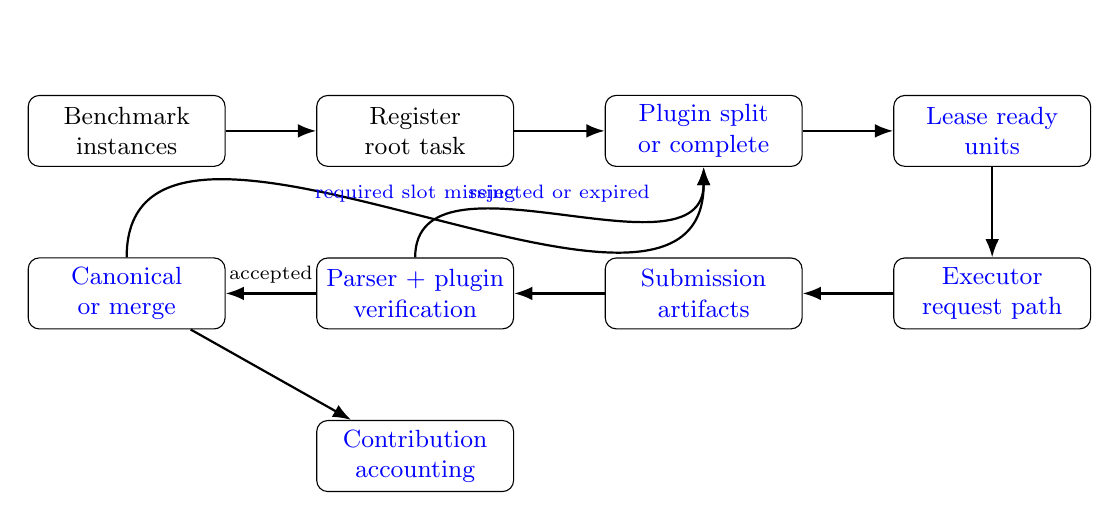
\begin{tikzpicture}[
  node distance=1.15cm,
  box/.style={draw, rounded corners, align=center, minimum width=2.5cm, minimum height=0.9cm, font=\small},
  smallbox/.style={draw, rounded corners, align=center, minimum width=2.2cm, minimum height=0.8cm, font=\small},
  arrow/.style={-Latex, thick}
]
\node[box] (bench) {Benchmark\\instances};
\node[box, right=of bench] (register) {Register\\root task};
\node[box, right=of register] (decompose) {\textcolor{blue}{Plugin split}\\\textcolor{blue}{or complete}};
\node[box, right=of decompose] (lease) {\textcolor{blue}{Lease ready}\\\textcolor{blue}{units}};
\node[box, below=of lease] (execute) {\textcolor{blue}{Executor}\\\textcolor{blue}{request path}};
\node[box, left=of execute] (submit) {\textcolor{blue}{Submission}\\\textcolor{blue}{artifacts}};
\node[box, left=of submit] (verify) {\textcolor{blue}{Parser + plugin}\\\textcolor{blue}{verification}};
\node[box, left=of verify] (merge) {\textcolor{blue}{Canonical}\\\textcolor{blue}{or merge}};
\node[box, below=of verify] (settle) {\textcolor{blue}{Contribution}\\\textcolor{blue}{accounting}};

\draw[arrow] (bench) -- (register);
\draw[arrow] (register) -- (decompose);
\draw[arrow] (decompose) -- (lease);
\draw[arrow] (lease) -- (execute);
\draw[arrow] (execute) -- (submit);
\draw[arrow] (submit) -- (verify);
\draw[arrow] (verify) -- node[above, font=\scriptsize] {accepted} (merge);
\draw[arrow] (merge) -- (settle);
\draw[arrow] (verify.north) to[out=90,in=270] node[above, font=\scriptsize] {\textcolor{blue}{rejected or expired}} (decompose.south);
\draw[arrow] (merge.north) to[out=90,in=270] node[above, font=\scriptsize] {\textcolor{blue}{required slot missing}} (decompose.south);
\end{tikzpicture}}
\caption{\textcolor{blue}{Common proof-of-concept workflow. Each benchmark instance is registered as a root task, optionally expanded by a plugin-owned split strategy, executed through an executor boundary, verified by a task-specific checker, and recorded through canonical, merge, contribution, and accounting events.}}
\label{fig:poc_workflow}
\end{figure}

\begin{table}[t]
\caption{How the two applications instantiate TokenShare.}
\label{tab:poc_applications}
\centering
\small
\begin{tabularx}{\linewidth}{p{0.18\linewidth}XX}
\toprule
Component & Large integer factorization & Lean formal proof production \\
\midrule
\textcolor{blue}{Root task} & \textcolor{blue}{Factor a small integer fixture, including prime and semiprime cases.} & \textcolor{blue}{Check a structured Lean theorem payload under fixed imports and environment $\Omega$.} \\
\textcolor{blue}{Task unit} & \textcolor{blue}{\texttt{root}, \texttt{factor\_integer}, \texttt{factor\_search\_range}, or \texttt{factorization\_merge}.} & \textcolor{blue}{Root theorem, child theorem, or merge-proof unit.} \\
\textcolor{blue}{Decomposition} & \textcolor{blue}{\texttt{candidate\_range\_partition.v1} covers $[2,\lfloor\sqrt n\rfloor]$ with required range slots.} & \textcolor{blue}{Lean-side deterministic split helper emits certificate-backed child goals and merge skeletons.} \\
\textcolor{blue}{Submission} & \textcolor{blue}{Structured range-result artifact or parser-failure evidence from raw output.} & \textcolor{blue}{Schema-bound proof candidate, checker report, proof artifact, and environment evidence.} \\
\textcolor{blue}{Verifier} & \textcolor{blue}{Deterministic arithmetic recheck and all-required merge policy.} & \textcolor{blue}{Fixed local Lean/lake checker with persisted stdout, stderr, generated source, and \texttt{EnvironmentRef}.} \\
\textcolor{blue}{Recovery} & \textcolor{blue}{Parser isolation, invalid-output rejection, expired lease requeue, and merge blocking.} & \textcolor{blue}{Rejected proof candidates remain evidence; accepted child proofs feed a checker-validated merge proof.} \\
\textcolor{blue}{Main metrics} & \textcolor{blue}{Final correctness, canonical pollution, completion, accounting, event count, artifact count.} & \textcolor{blue}{Real checker evidence, environment completeness, decomposition/merge lifecycle coverage.} \\
\bottomrule
\end{tabularx}
\end{table}


\subsection{Application I: Large Integer Factorization}

{\color{blue}
The first proof-of-concept application is the \texttt{factorization@0.1.0} plugin. Its role is not to compete with specialized number-theory software; it supplies a compact workload in which the protocol can observe typed decomposition, bounded execution, deterministic verification, all-required merge, contribution accounting, and canonical-state safety.
}

\paragraph{Task specification.}
{\color{blue}
The registered task is
\[
\mathcal{S}_{\mathrm{fac}}=(n,\mathrm{requested\_output},\mathrm{params},\mathrm{plugin\_version}),
\]
where $n$ is stored as a decimal string and the requested output is a prime factorization result. A range child accepts only \texttt{factorization.range\_result.v1}. The core arithmetic check is
\[
V_{\mathrm{fac}}(n,d)=
\begin{cases}
1, & \text{if } 1<d<n \text{ and } n\bmod d=0,\\
0, & \text{otherwise}.
\end{cases}
\]
and no-factor claims are also rechecked against their assigned closed interval. The plugin merge policy emits a final \texttt{PrimeFactorizationResult} only when the required evidence is complete.
}

\paragraph{Decomposition.}
{\color{blue}
The plugin split strategy partitions the candidate divisor interval $[2,\lfloor \sqrt{n}\rfloor]$ into ranges
\[
I_j=[a_j,b_j],
\]
with a coverage proof showing no gaps and no overlaps. Each range unit receives a bounded instruction:
\[
u_j=(n,[a_j,b_j],\mathrm{coverage\_id},\mathrm{child\_index}).
\]
The executor may search only inside that interval and may not create child tasks, invent output schemas, or claim the final factorization.
}

\paragraph{Experimental workflow.}
{\color{blue}
Experiment~1 runs small-prime, prime-range, semiprime-range, and extended semiprime fixture cases. Experiment~2 injects invalid factor, false no-factor, raw-only parse failure, expired lease, and verification-budget failures. Experiment~3 disables one boundary per run to show controlled degradation.
}

\paragraph{Baselines and metrics.}
{\color{blue}
The primary baseline is not a faster factorization algorithm but the same fixture lifecycle with selected protocol boundaries removed. Metrics therefore focus on final correctness, completion rate, canonical pollution, accounting success, event footprint, and artifact footprint.
}


\subsection{Application II: Lean Formal Proof Production}

{\color{blue}
The second proof-of-concept application is the \texttt{lean\_proof@0.1.0} plugin. Lean supplies a high-value verification boundary: a proof artifact is accepted only if a fixed local Lean/lake environment checks it and the resulting checker evidence is persisted. This makes Lean a strong test for whether TokenShare can coordinate a domain whose correctness is external to the protocol core.
}

\paragraph{Task specification.}
{\color{blue}
The registered task is
\[
\mathcal{S}_{\mathrm{Lean}}=(s,\mathcal{I},\Omega,\Pi),
\]
where $s$ is a structured theorem statement, $\mathcal{I}$ is the allowed import set, $\Omega$ is the fixed Lean/lake environment, and $\Pi$ is the decomposition policy. A proof candidate must bind to the theorem payload digest. The checker predicate is
\[
V_{\mathrm{Lean}}(s,y,\Omega)=
\begin{cases}
1, & \text{if the project builds successfully in } \Omega,\\
0, & \text{otherwise}.
\end{cases}
\]
and an accepted report must include logs, generated source, proof artifact, and \texttt{EnvironmentRef}.
}

\paragraph{Recursive decomposition.}
{\color{blue}
Each Lean task unit is represented by a structured theorem payload rather than a natural-language goal. Direct proof and decomposition/merge paths are both supported in the fixture suite. A decomposition result is accepted only if the Lean-side helper emits a supported split certificate:
\[
u=(s,\mathcal{I},\Omega,\mathrm{payload\_digest},\Pi),
\]
and a proof candidate may enter the protocol only as one of the following artifact-backed forms:
\[
y_u \in \{\textsc{DirectProof}(p_u),\textsc{ChildProof}(p_i),\textsc{MergeProof}(p_{\mathrm{root}})\}.
\]
The merge policy reads accepted child proof artifacts, constructs a root merge proof, and invokes the checker again.
}

\paragraph{Experimental workflow.}
{\color{blue}
Experiment~4 runs a factorization semiprime lifecycle, a Lean direct proof fixture, and a Lean decomposition/merge fixture under the same experiment runner. The Lean adapter first performs a real preflight check, then reports checker evidence and environment completeness.
}


\paragraph{\textcolor{blue}{Recovery and accounting.}}
{\color{blue}
Lean proof evidence enters the same accounting path as factorization evidence: accepted canonical proof artifacts and accepted merge facts can produce eligible contribution records, and root completion can trigger an accounting batch. Invalid proof candidates remain auditable checker evidence but do not bind canonical state.
}

\paragraph{Baselines and metrics.}
{\color{blue}
The Lean cases are evaluated by real checker evidence, environment-reference completeness, canonical pollution, event footprint, artifact footprint, and whether direct and decomposition/merge paths complete through the shared protocol lifecycle.
}



}
% Experiment section rewritten from regenerated outputs/experiments artifacts.
\begingroup
\color{blue}
\small
\renewcommand{\arraystretch}{1.12}
\providecommand{\FloatBarrier}{}
\providecommand{\TS}{TokenShare}
\providecommand{\tickyes}{\(\checkmark\)}
\providecommand{\tickno}{--}

\tikzset{
  tsbox/.style={draw=blue!70!black, fill=blue!6, rounded corners=2pt, line width=0.4pt},
  tsdarkbox/.style={draw=blue!70!black, fill=blue!18, rounded corners=2pt, line width=0.4pt},
  tsline/.style={draw=blue!70!black, line width=0.5pt},
  tsarrow/.style={draw=blue!70!black, -stealth, line width=0.6pt},
  tslabel/.style={font=\scriptsize, text=blue!75!black},
  tssmall/.style={font=\tiny, text=blue!75!black}
}

% Make caption labels such as "Figure 1:" and "Table 1:" blue as well.
% This avoids the common problem where only the caption body is blue but
% the automatically generated label remains black.
\makeatletter
\let\TSoldmakecaption\@makecaption
\renewcommand{\@makecaption}[2]{%
  \vskip\abovecaptionskip
  \sbox\@tempboxa{{\color{blue}\small #1: #2}}%
  \ifdim \wd\@tempboxa >\hsize
    {\color{blue}\small #1: #2\par}%
  \else
    \global\@minipagefalse
    \hb@xt@\hsize{\hfil\box\@tempboxa\hfil}%
  \fi
  \vskip\belowcaptionskip}
\makeatother

\section{Experiments}
\label{sec:experiments}

\subsection{Evaluation Objective}
\label{subsec:evaluation-objective}

{\color{blue}
The experiments evaluate whether TokenShare works as a concept, not whether the prototype is an optimized factorization engine or theorem prover. Each experiment asks a different question about shared tokenized capacity: Can it be turned into a complete useful output? Can bad contributions be rejected without polluting shared state? Are the protocol boundaries necessary? Can the same sharing mechanism survive a change of task domain?

The implementation supplies the measurement instrument. We organize the evaluation into four experiments. Experiment~1 tests whether a real factorization plugin can convert shared execution units into a verified final result. Experiment~2 injects invalid or incomplete submissions to test whether rejected expenditure remains evidence rather than contribution. Experiment~3 disables individual protections to test whether TokenShare depends on parser ownership, verification, requeue, merge gates, and slot integrity. Experiment~4 tests whether the same contribution lifecycle generalizes from arithmetic search to real Lean proof production. We then report an auxiliary contributor-heterogeneity simulation that compares deterministic local, real model-backed, and malformed contributors on the same semiprime task.
}

\begin{table}[!htbp]
\centering
\caption{\textcolor{blue}{Evaluation groups as evidence for the TokenShare concept. The AI executor profile is treated as an auxiliary contributor-heterogeneity simulation rather than a separate experiment.}}
\label{tab:evaluation-groups}
\small
{\color{blue}
\begin{tabularx}{\linewidth}{p{0.17\linewidth}p{0.25\linewidth}X}
\toprule
Group & Setting & Conceptual claim \\
\midrule
Experiment 1 & Factorization lifecycle
& Shared bounded compute can become a verified final contribution through decomposition, execution, verification, merge, contribution recording, and accounting. \\
Experiment 2 & Failure recovery
& Invalid factors, false no-factor claims, parse failures, crashes, and
verification-budget failures are isolated or recovered without canonical
pollution. \\
Experiment 3 & Mechanism ablation
& Removing verifier, parser policy, requeue, merge gate, or slot-integrity checks breaks the conversion from spent capacity to accepted contribution. \\
Experiment 4 & Cross-plugin generality
& TokenShare is not tied to one task: arithmetic search and formal proof production share the same contribution lifecycle while preserving plugin-owned semantics. \\
Auxiliary simulation & Heterogeneous contributors
& Model tokens, local compute, and malformed outputs can enter the same system, but only verified evidence becomes useful contribution. \\
\bottomrule
\end{tabularx}
}
\end{table}

\subsection{Metrics and Status Definitions}
\label{subsec:metrics-status}

{\color{blue}
We report metrics at two levels. Task-level metrics tell us whether the useful work was actually done: final correctness, parser success rate, parsed output count, and parse failure count. TokenShare-level metrics tell us whether spent capacity became trustworthy contribution: completion rate, canonical pollution count, accounting success, real checker evidence, event count, artifact count, provider attempts, retry count, token usage, cost estimate, and latency. We use \emph{passed} for a run that satisfies the expected property, \emph{failed} for an unexpected violation, \emph{blocked} for an unavailable runtime dependency, and \emph{inconclusive} for an intentional ablation run in which disabling a protection causes the expected degradation.
}

\subsection{Reproducibility and Setting Artifacts}
\label{subsec:experiment-settings-artifacts}

{\color{blue}
Before reporting results, we regenerated the experiment output tree from a clean
\texttt{outputs/experiments} directory.  The settings are not reconstructed from
the prose of this paper; they are persisted next to the results.  This is
important for TokenShare because a contribution economy must make the conditions
under which evidence was produced visible: seed, fixture identity, plugin and
executor identities, failure profile, ablation mode, request limits, parser
policy, provider selection digest, and artifact paths are part of the audit
surface.
}

\begin{table}[!htbp]
\centering
\caption{\textcolor{blue}{Regenerated setting and result artifacts used by the
experiment section.}}
\label{tab:experiment-setting-artifacts}
\small
{\color{blue}
\begin{tabularx}{\linewidth}{p{0.33\linewidth}p{0.25\linewidth}X}
\toprule
Artifact & Role & Contents used in the paper \\
\midrule
\url{outputs/experiments/phase8_experiment_settings.json}
& Experiment 1--4 settings
& Seed \(1\), 17 experiment cases, fixture names, plugin versions, expected
outputs, fault profiles, ablation modes, profile digests, and per-run manifest
paths. \\
\url{outputs/experiments/phase8_suite_report.json}
& Experiment 1--4 suite result
& Total, passed, inconclusive, failed, and blocked run counts; summary and
settings paths; local AI config digest without secrets. \\
\url{outputs/experiments/phase8_suite_summary.csv}
& Paper table source
& Per-case status, correctness, canonical pollution, completion, settlement,
real checker evidence, event count, and artifact count. \\
\url{outputs/experiments/runs/*/run_manifest.json}
& Run-level setting/evidence link
& Frozen plugin and executor descriptors, seed, clock semantics, event-log ref,
artifact root, status, and replayable run identity. \\
\url{outputs/experiments/ai_profile_real/ai_profile_settings.json}
& Auxiliary AI-profile settings
& Real-transport flag, request limits \texttt{max\_tokens=1024} and
\texttt{timeout\_seconds=30},
JSON-mode parser policy, semiprime range inputs, config digest, entry metadata,
and strict-arithmetic model filter. \\
\url{outputs/experiments/ai_profile_real/ai_profile_suite_report.json}
& Auxiliary AI-profile result
& Deterministic, real model-backed, and malformed raw-output profiles with raw,
parsed, parse-failure, usage, cost, latency, provider, and model evidence. \\
\bottomrule
\end{tabularx}
}
\end{table}

\subsection{Suite-Level Results}
\label{subsec:suite-level-results}

{\color{blue}
The default suite contains 17 runs. Twelve runs pass, five runs are expected ablation degradations, and no run fails or becomes blocked. This suite-level result matters because TokenShare is evaluated as a contribution system: the passing runs show that shared capacity can be converted into accepted work, while the inconclusive ablation runs show that the conversion depends on specific protections rather than on final-answer luck.
}

\begin{figure}[!htbp]
\centering
{\color{blue}
\begin{tikzpicture}[x=1cm,y=1cm]
  \node[tslabel, anchor=west] at (0,2.35) {Default suite status};

  % Main ribbon.
  % Total width = 12cm.
  % 17 runs total: 12 passed -> 8.47cm, 5 inconclusive -> 3.53cm.
  \draw[tsline] (0,1.40) rectangle (12,1.90);
  \fill[blue!22] (0,1.40) rectangle (8.47,1.90);
  \fill[blue!8]  (8.47,1.40) rectangle (12,1.90);
  \draw[tsline] (8.47,1.40) -- (8.47,1.90);

  \node[tslabel] at (4.24,1.65) {12 passed};
  \node[tslabel] at (10.24,1.65) {5 inconclusive};

  % Tick marks and labels.
  \draw[tsline] (0,1.28) -- (0,1.12);
  \draw[tsline] (8.47,1.28) -- (8.47,1.12);
  \draw[tsline] (12,1.28) -- (12,1.12);

  \node[tssmall, anchor=north] at (0,1.05) {0};
  \node[tssmall, anchor=north] at (8.47,1.05) {12};
  \node[tssmall, anchor=north] at (12,1.05) {17};

  % Summary cards, placed lower and separated.
  \node[tsbox, minimum width=2.7cm, minimum height=0.58cm] at (1.35,0.35) {Failed: 0};
  \node[tsbox, minimum width=2.7cm, minimum height=0.58cm] at (4.65,0.35) {Blocked: 0};
  \node[tsbox, minimum width=4.8cm, minimum height=0.58cm] at (9.10,0.35) {Ablation degradations: 5};
\end{tikzpicture}
}
\caption{\textcolor{blue}{Suite-level status ribbon. The default suite has 17 runs: 12 passed, 5 intentional ablation degradations, 0 failed, and 0 blocked.}}
\label{fig:suite-status-ribbon}
\end{figure}

\FloatBarrier

\subsection{Experiment 1: End-to-End Factorization Lifecycle}
\label{subsec:exp1-factorization}

{\color{blue}
\textbf{Purpose.} Experiment~1 asks whether TokenShare can turn shared bounded compute into a complete verified output. The purpose is not to benchmark factorization; factorization is a compact domain in which decomposition, execution, verification, merge, and accounting are all checkable.

\textbf{Setting.} The setting uses the real \texttt{factorization@0.1.0} plugin. The four cases cover direct completion, prime-range verification, semiprime decomposition, and a larger semiprime benchmark. Contributors execute bounded range-search units; the plugin owns parsing, range verification, and all-required merge.

\textbf{Result and interpretation.} All four cases pass with final correctness, completion rate 1.0, accounting success, and zero canonical pollution. The result shows the basic TokenShare promise: a large useful task can be split into shareable units, each unit can produce evidence, and accepted child evidence can be merged into a final result with a replayable contribution trail.
}

\begin{table}[!htbp]
\centering
\caption{\textcolor{blue}{Experiment 1: factorization lifecycle results.}}
\label{tab:factorization-results}
\small
{\color{blue}
\begin{tabularx}{\linewidth}{p{0.10\linewidth}p{0.18\linewidth}p{0.14\linewidth}>{\centering\arraybackslash}p{0.10\linewidth}>{\centering\arraybackslash}p{0.10\linewidth}X}
\toprule
Case & Instance & Output & Events & Artifacts & Interpretation \\
\midrule
E1a & \(N=2\) & \([2]\) & 22 & 9
& Direct completion without range expansion. \\
E1b & \(N=97\) & \([97]\) & 96 & 38
& Prime case completed through bounded range verification. \\
E1c & \(N=91\) & \([7,13]\) & 96 & 38
& Semiprime case completed through range search and all-required merge. \\
E1d & \(N=8051\) & \([83,97]\) & 148 & 62
& Larger semiprime case exercised the same lifecycle at greater evidence depth. \\
\bottomrule
\end{tabularx}
}
\end{table}

\begin{figure}[!htbp]
\centering
{\color{blue}
\begin{tikzpicture}[x=0.085cm,y=0.82cm]
  \node[tslabel, anchor=west] at (0,4.85) {Evidence footprint by case};

  % axis
  \draw[tsline] (0,0) -- (160,0);
  \foreach \x/\lab in {0/0,40/40,80/80,120/120,160/160} {
    \draw[tsline] (\x,0.04) -- (\x,-0.04);
    \node[tssmall, anchor=north] at (\x,-0.08) {\lab};
  }
  \node[tssmall, anchor=west] at (162,0) {count};

  % rows: label, events, artifacts
  \foreach \y/\case/\ev/\art in {
    4/E1a/22/9,
    3/E1b/96/38,
    2/E1c/96/38,
    1/E1d/148/62
  }{
    \node[tslabel, anchor=east] at (-4,\y) {\case};
    \draw[blue!15, line width=4pt] (0,\y) -- (160,\y);
    \draw[blue!35, line width=4pt] (0,\y+0.08) -- (\ev,\y+0.08);
    \filldraw[draw=blue!70!black, fill=blue!35] (\ev,\y+0.08) circle (2.2pt);
    \node[tssmall, anchor=west] at (\ev+3,\y+0.08) {events \ev};

    \draw[blue!20, line width=4pt] (0,\y-0.12) -- (\art,\y-0.12);
    \filldraw[draw=blue!70!black, fill=blue!10] (\art,\y-0.12) circle (2pt);
    \node[tssmall, anchor=west] at (\art+3,\y-0.12) {artifacts \art};
  }
\end{tikzpicture}
}
\caption{\textcolor{blue}{Lollipop-style evidence footprint for Experiment~1. E1d produces the largest event and artifact footprint, while all four cases preserve final correctness and zero canonical pollution.}}
\label{fig:factorization-lollipop}
\end{figure}

{\color{blue}
The semiprime cases are the most informative because they require multiple child range results, verified canonical bindings, and a plugin-owned merge rule. They demonstrate that TokenShare is not merely recording a final answer; it is recording how distributed expenditure becomes accepted contribution.
}

\FloatBarrier

\subsection{Experiment 2: Failure Injection and Recovery}
\label{subsec:exp2-failure}

{\color{blue}
\textbf{Purpose.} Experiment~2 asks whether failed or malicious token expenditure can be prevented from becoming shared contribution. This is essential for TokenShare: a system that pools capacity but cannot reject bad evidence would only amplify error.

\textbf{Setting.} Each run injects one failure mode into the same factorization contribution lifecycle: an invalid factor, a false no-factor claim, an unparsable raw output, a worker crash or expired lease, and an over-budget no-factor recheck.

\textbf{Result and interpretation.} All five cases pass with final correctness, completion rate 1.0, accounting success, and zero canonical pollution. The result shows that TokenShare preserves bad expenditure as audit evidence without allowing it to become accepted contribution. Parser failures, verifier rejections, lease recovery, and budget limits are not engineering decorations; they are the safeguards that make sharing useful capacity credible.
}

\begin{figure}[!htbp]
\centering
{\color{blue}
\resizebox{0.92\linewidth}{!}{%
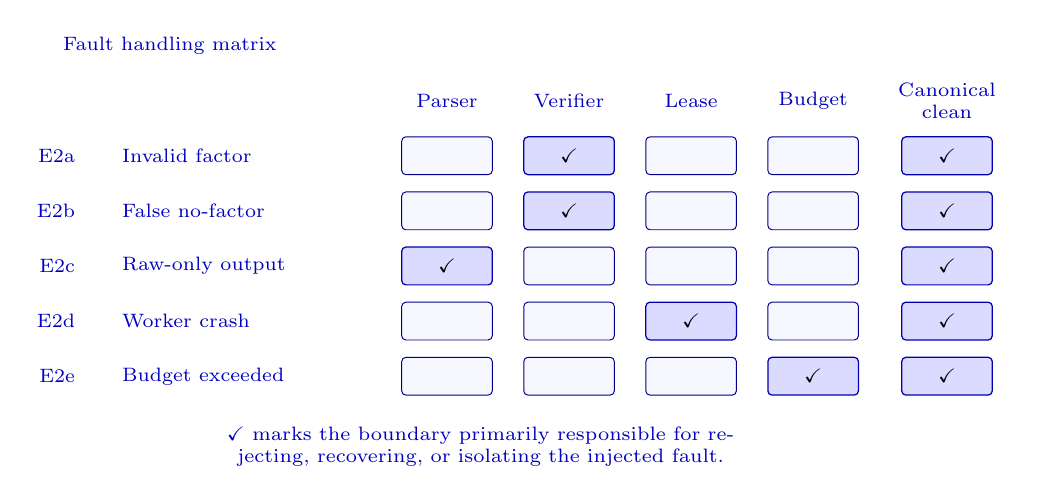
\begin{tikzpicture}[
  font=\scriptsize,
  rowlabel/.style={
    text=blue!75!black,
    anchor=east
  },
  faultlabel/.style={
    text=blue!75!black,
    anchor=west
  },
  header/.style={
    text=blue!75!black,
    align=center
  },
  cell/.style={
    draw=blue!55!black,
    fill=blue!3,
    rounded corners=1.5pt,
    line width=0.35pt,
    minimum width=1.15cm,
    minimum height=0.48cm,
    align=center
  },
  hitcell/.style={
    draw=blue!70!black,
    fill=blue!14,
    rounded corners=1.5pt,
    line width=0.45pt,
    minimum width=1.15cm,
    minimum height=0.48cm,
    align=center
  }
]

% Title
\node[
  font=\scriptsize,
  text=blue!75!black,
  anchor=west
] at (-5.4,3.55)
{Fault handling matrix};

% Column headers
\node[header] at (-0.4,2.85) {Parser};
\node[header] at (1.15,2.85) {Verifier};
\node[header] at (2.70,2.85) {Lease};
\node[header] at (4.25,2.85) {Budget};
\node[header, text width=1.65cm] at (5.95,2.85) {Canonical\\clean};

% ---------------- Row E2a ----------------
\node[rowlabel] at (-5.0,2.15) {E2a};
\node[faultlabel] at (-4.65,2.15) {Invalid factor};

\node[cell] at (-0.4,2.15) {};
\node[hitcell] at (1.15,2.15) {\(\checkmark\)};
\node[cell] at (2.70,2.15) {};
\node[cell] at (4.25,2.15) {};
\node[hitcell] at (5.95,2.15) {\(\checkmark\)};

% ---------------- Row E2b ----------------
\node[rowlabel] at (-5.0,1.45) {E2b};
\node[faultlabel] at (-4.65,1.45) {False no-factor};

\node[cell] at (-0.4,1.45) {};
\node[hitcell] at (1.15,1.45) {\(\checkmark\)};
\node[cell] at (2.70,1.45) {};
\node[cell] at (4.25,1.45) {};
\node[hitcell] at (5.95,1.45) {\(\checkmark\)};

% ---------------- Row E2c ----------------
\node[rowlabel] at (-5.0,0.75) {E2c};
\node[faultlabel] at (-4.65,0.75) {Raw-only output};

\node[hitcell] at (-0.4,0.75) {\(\checkmark\)};
\node[cell] at (1.15,0.75) {};
\node[cell] at (2.70,0.75) {};
\node[cell] at (4.25,0.75) {};
\node[hitcell] at (5.95,0.75) {\(\checkmark\)};

% ---------------- Row E2d ----------------
\node[rowlabel] at (-5.0,0.05) {E2d};
\node[faultlabel] at (-4.65,0.05) {Worker crash};

\node[cell] at (-0.4,0.05) {};
\node[cell] at (1.15,0.05) {};
\node[hitcell] at (2.70,0.05) {\(\checkmark\)};
\node[cell] at (4.25,0.05) {};
\node[hitcell] at (5.95,0.05) {\(\checkmark\)};

% ---------------- Row E2e ----------------
\node[rowlabel] at (-5.0,-0.65) {E2e};
\node[faultlabel] at (-4.65,-0.65) {Budget exceeded};

\node[cell] at (-0.4,-0.65) {};
\node[cell] at (1.15,-0.65) {};
\node[cell] at (2.70,-0.65) {};
\node[hitcell] at (4.25,-0.65) {\(\checkmark\)};
\node[hitcell] at (5.95,-0.65) {\(\checkmark\)};

% Bottom note
\node[
  font=\scriptsize,
  text=blue!75!black,
  align=center,
  text width=10.8cm
] at (0,-1.55)
{\(\checkmark\) marks the boundary primarily responsible for rejecting,
recovering, or isolating the injected fault.};

\end{tikzpicture}
}
}
\caption{\textcolor{blue}{Failure-handling matrix for Experiment~2. Each injected failure is handled by the relevant protocol boundary, and every case preserves zero canonical pollution.}}
\label{fig:failure-handling-matrix}
\end{figure}

{\color{blue}
These results show that executor submission is not equivalent to contribution. A candidate output must pass the parser, verifier, and canonical-selection boundary before it can affect accepted state. Invalid evidence may remain auditable, but it does not become canonical evidence.
}

\FloatBarrier

\subsection{Experiment 3: Mechanism Ablation}
\label{subsec:exp3-ablation}

{\color{blue}
\textbf{Purpose.} Experiment~3 asks which mechanisms are necessary for TokenShare to work as a sharing concept. If a mechanism can be removed without consequence, it is not central to the claim; if removal causes predictable degradation, it marks a real boundary in the conversion from resource expenditure to accepted contribution.

\textbf{Setting.} Each run disables one protection: verification, parser policy, requeue, all-required merge gate, or slot-integrity checking. The expected outcome is controlled degradation, not normal completion.

\textbf{Result and interpretation.} All five ablations are reported as inconclusive by design, with completion rate 0.0 and no accounting success. The verifier ablation additionally produces one canonical pollution event, showing the direct risk of bypassing plugin verification. This establishes that TokenShare depends on a bundle of boundaries: parser ownership, verifier authority, lease recovery, merge readiness, and slot integrity.
}

\begin{figure}[!htbp]
\centering
{\color{blue}
\begin{tikzpicture}[x=1.05cm,y=0.72cm]
  \node[tslabel, anchor=west] at (0,6.1) {Ablation outcome heatmap};

  \node[tssmall] at (4.1,5.35) {Completion};
  \node[tssmall] at (5.9,5.35) {Accounting};
  \node[tssmall] at (7.6,5.35) {Pollution};
  \node[tssmall] at (9.4,5.35) {Risk signal};

  \foreach \row/\case/\removed/\comp/\settle/\poll/\risk in {
    4.6/E3a/Verifier/0/0/1/Canonical,
    3.8/E3b/Parser policy/0/0/0/Raw boundary,
    3.0/E3c/Requeue/0/0/0/Stuck work,
    2.2/E3d/Merge gate/0/0/0/Premature merge,
    1.4/E3e/Slot check/0/0/0/Wrong slot
  }{
    \node[tslabel, anchor=east] at (1.1,\row) {\case};
    \node[tssmall, anchor=west] at (1.25,\row) {\removed};

    \node[tsbox, minimum width=0.7cm, minimum height=0.40cm] at (4.1,\row) {0.0};
    \node[tsbox, minimum width=0.7cm, minimum height=0.40cm] at (5.9,\row) {no};

    \ifnum\poll=1
      \node[tsdarkbox, minimum width=0.7cm, minimum height=0.40cm] at (7.6,\row) {1};
    \else
      \node[tsbox, minimum width=0.7cm, minimum height=0.40cm] at (7.6,\row) {0};
    \fi

    \node[tsbox, minimum width=2.45cm, minimum height=0.40cm] at (9.4,\row) {\risk};
  }

  \node[tssmall, anchor=west] at (0.8,0.45)
  {All ablations are inconclusive by design; E3a directly shows canonical pollution when verification is removed.};
\end{tikzpicture}
}
\caption{\textcolor{blue}{Mechanism-ablation heatmap. Removing core protections prevents normal completion; removing verification additionally creates canonical pollution.}}
\label{fig:ablation-heatmap}
\end{figure}

{\color{blue}
The ablation suite supports a mechanism-level claim: useful sharing is not a property of the task solver alone, but of the solver together with parser ownership, verification, lease recovery, merge gating, and slot integrity.
}

\FloatBarrier

\subsection{Experiment 4: Cross-Plugin Generality}
\label{subsec:exp4-cross-plugin}

{\color{blue}
\textbf{Purpose.} Experiment~4 asks whether TokenShare is a general concept or merely a factorization workflow. A credible sharing mechanism should let different domains define their own valid contributions while using the same coordination and evidence lifecycle.

\textbf{Setting.} The experiment runs three real-plugin cases: a factorization semiprime lifecycle, a Lean direct proof, and a Lean decomposition/merge proof. The Lean cases use real checker evidence from a fixed local Lean/lake environment, including proof artifacts, logs, and environment references.

\textbf{Result and interpretation.} The factorization case and both Lean proof cases pass. This result supports the cross-domain claim: TokenShare can coordinate different forms of tokenized capacity, from bounded arithmetic compute to formal proof attempts, while keeping domain semantics inside plugins and keeping contribution evidence in a shared protocol lifecycle.
}

\begin{figure}[!htbp]
\centering
{\color{blue}
\resizebox{0.92\linewidth}{!}{%
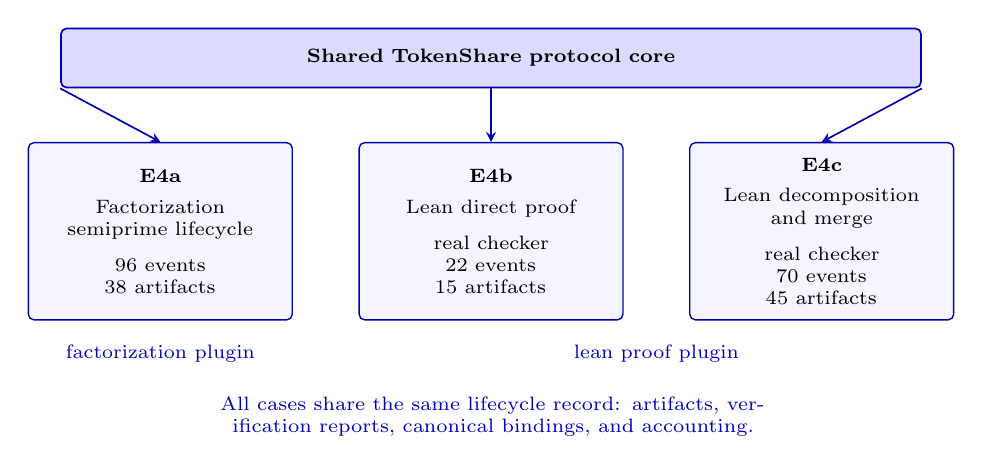
\begin{tikzpicture}[
  font=\scriptsize,
  box/.style={
    draw=blue!70!black,
    fill=blue!4,
    rounded corners=2pt,
    line width=0.5pt,
    align=center,
    inner sep=5pt
  },
  corebox/.style={
    draw=blue!70!black,
    fill=blue!14,
    rounded corners=2pt,
    line width=0.6pt,
    align=center,
    inner sep=6pt
  },
  arrow/.style={
    draw=blue!70!black,
    -stealth,
    line width=0.6pt
  }
]

% Top core box
\node[corebox, text width=10.5cm, minimum height=0.75cm] (core) at (0,3.2)
{\textbf{Shared TokenShare protocol core}};

% Three case cards
\node[box, text width=3.0cm, minimum height=2.25cm] (e4a) at (-4.2,1.0)
{\textbf{E4a}\\[3pt]
Factorization\\
semiprime lifecycle\\[5pt]
96 events\\
38 artifacts};

\node[box, text width=3.0cm, minimum height=2.25cm] (e4b) at (0,1.0)
{\textbf{E4b}\\[3pt]
Lean direct proof\\[5pt]
real checker\\
22 events\\
15 artifacts};

\node[box, text width=3.0cm, minimum height=2.25cm] (e4c) at (4.2,1.0)
{\textbf{E4c}\\[3pt]
Lean decomposition\\
and merge\\[5pt]
real checker\\
70 events\\
45 artifacts};

% Plugin labels
\node[font=\scriptsize, text=blue!75!black] at (-4.2,-0.55)
{factorization plugin};

\node[font=\scriptsize, text=blue!75!black] at (2.1,-0.55)
{lean proof plugin};

% Arrows from core to cases
\draw[arrow] (core.south west) -- (e4a.north);
\draw[arrow] (core.south) -- (e4b.north);
\draw[arrow] (core.south east) -- (e4c.north);

% Bottom note
\node[
  font=\scriptsize,
  text=blue!75!black,
  align=center,
  text width=10.5cm
] at (0,-1.35)
{All cases share the same lifecycle record: artifacts, verification reports,
canonical bindings, and accounting.};

\end{tikzpicture}
}
}
\caption{\textcolor{blue}{Cross-plugin generality in Experiment~4. The same TokenShare contribution lifecycle supports both factorization and Lean proof plugins while domain semantics remain plugin-owned.}}
\label{fig:cross-plugin-map}
\end{figure}

\begin{table}[!htbp]
\centering
\caption{\textcolor{blue}{Experiment 4: cross-plugin generality results.}}
\label{tab:cross-plugin-results}
\footnotesize
{\color{blue}
\begin{tabularx}{0.96\linewidth}{
  @{}
  >{\raggedright\arraybackslash}p{0.10\linewidth}
  >{\raggedright\arraybackslash}p{0.24\linewidth}
  >{\raggedright\arraybackslash}p{0.22\linewidth}
  >{\raggedright\arraybackslash}X
  @{}
}
\toprule
Case & Workload and plugin & Evidence footprint & Interpretation \\
\midrule

E4a
&
\begin{minipage}[t]{\linewidth}
\textbf{Semiprime lifecycle}

Plugin: factorization
\end{minipage}
&
\begin{minipage}[t]{\linewidth}
Checker evidence: no

Events: 96

Artifacts: 38
\end{minipage}
&
\begin{minipage}[t]{\linewidth}
The arithmetic-search plugin completes the shared TokenShare lifecycle through plugin-owned factorization semantics.
\end{minipage}
\\[1.0em]

E4b
&
\begin{minipage}[t]{\linewidth}
\textbf{Lean direct proof}

Plugin: lean proof
\end{minipage}
&
\begin{minipage}[t]{\linewidth}
Checker evidence: yes

Events: 22

Artifacts: 15
\end{minipage}
&
\begin{minipage}[t]{\linewidth}
The direct proof path is accepted by a real Lean checker, showing that protocol acceptance can rely on external formal verification evidence.
\end{minipage}
\\[1.0em]

E4c
&
\begin{minipage}[t]{\linewidth}
\textbf{Lean decomposition and merge}

Plugin: lean proof
\end{minipage}
&
\begin{minipage}[t]{\linewidth}
Checker evidence: yes

Events: 70

Artifacts: 45
\end{minipage}
&
\begin{minipage}[t]{\linewidth}
The split child proofs and the merged root proof are accepted by the checker, demonstrating that the protocol can coordinate decomposition and merge beyond direct proof submission.
\end{minipage}
\\

\bottomrule
\end{tabularx}
}
\end{table}
{\color{blue}
The result supports the TokenShare generality claim. The common system records lifecycle state, artifacts, verification reports, canonical bindings, and accounting records, while factorization arithmetic and Lean proof checking remain outside the protocol core. TokenShare shares capacity and evidence; each domain still defines what valid work means.
}

\FloatBarrier

\subsection{Auxiliary Simulation: Heterogeneous Contributors}
\label{subsec:aux-heterogeneous-contributors}

{\color{blue}
The auxiliary simulation connects the experiments back to the motivating idea of sharing tokens. It is not a fifth experiment; it approximates a multi-user setting by running the same semiprime task under three contributor profiles: a deterministic local contributor, a real model-backed contributor, and a malformed raw-output contributor. The workload is \(N=91\), with expected factors \([7,13]\).

The simulation tests whether different resource media can enter TokenShare through the same contribution boundary. The model-backed contributor spends real API/model capacity, but the protocol does not directly trust raw responses. The malformed profile models a contributor whose expenditure produces evidence but no accepted contribution. Thus the simulation distinguishes resource spending from useful sharing: only parsed and verified evidence can count.
}

\begin{figure}[!htbp]
\centering
{\color{blue}
\resizebox{0.92\linewidth}{!}{%
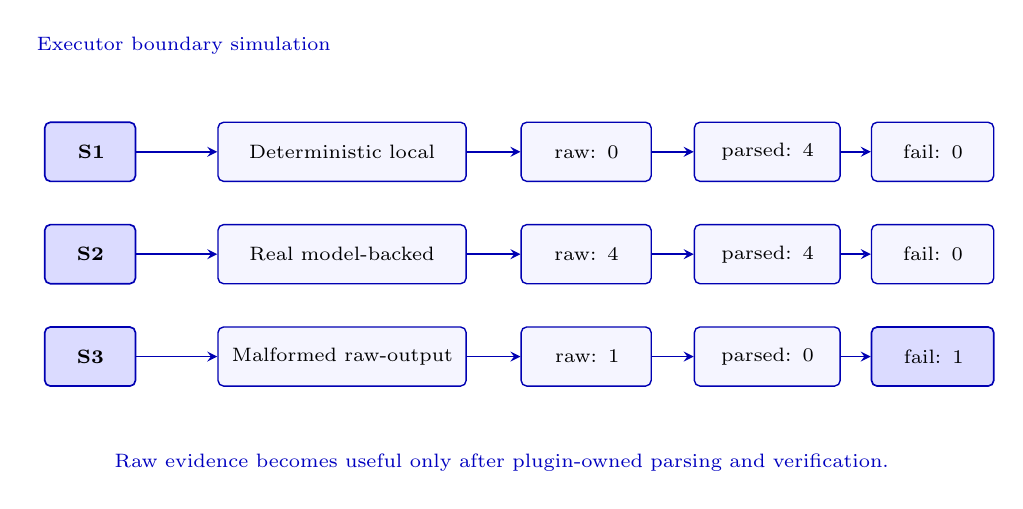
\begin{tikzpicture}[
  font=\scriptsize,
  box/.style={
    draw=blue!70!black,
    fill=blue!4,
    rounded corners=2pt,
    line width=0.5pt,
    align=center,
    inner sep=5pt
  },
  darkbox/.style={
    draw=blue!70!black,
    fill=blue!14,
    rounded corners=2pt,
    line width=0.6pt,
    align=center,
    inner sep=5pt
  },
  arrow/.style={
    draw=blue!70!black,
    -stealth,
    line width=0.6pt
  }
]

% Title
\node[font=\scriptsize, text=blue!75!black, anchor=west] at (-5.4,3.25)
{Executor boundary simulation};

% Row 1
\node[darkbox, text width=0.8cm, minimum height=0.75cm] (s1id) at (-4.6,1.9)
{\textbf{S1}};

\node[box, text width=2.8cm, minimum height=0.75cm] (s1type) at (-1.4,1.9)
{Deterministic local};

\node[box, text width=1.3cm, minimum height=0.75cm] (s1raw) at (1.7,1.9)
{raw: 0};

\node[box, text width=1.5cm, minimum height=0.75cm] (s1parsed) at (4.0,1.9)
{parsed: 4};

\node[box, text width=1.2cm, minimum height=0.75cm] (s1fail) at (6.1,1.9)
{fail: 0};

% Row 2
\node[darkbox, text width=0.8cm, minimum height=0.75cm] (s2id) at (-4.6,0.6)
{\textbf{S2}};

\node[box, text width=2.8cm, minimum height=0.75cm] (s2type) at (-1.4,0.6)
{Real model-backed};

\node[box, text width=1.3cm, minimum height=0.75cm] (s2raw) at (1.7,0.6)
{raw: 4};

\node[box, text width=1.5cm, minimum height=0.75cm] (s2parsed) at (4.0,0.6)
{parsed: 4};

\node[box, text width=1.2cm, minimum height=0.75cm] (s2fail) at (6.1,0.6)
{fail: 0};

% Row 3
\node[darkbox, text width=0.8cm, minimum height=0.75cm] (s3id) at (-4.6,-0.7)
{\textbf{S3}};

\node[box, text width=2.8cm, minimum height=0.75cm] (s3type) at (-1.4,-0.7)
{Malformed raw-output};

\node[box, text width=1.3cm, minimum height=0.75cm] (s3raw) at (1.7,-0.7)
{raw: 1};

\node[box, text width=1.5cm, minimum height=0.75cm] (s3parsed) at (4.0,-0.7)
{parsed: 0};

\node[darkbox, text width=1.2cm, minimum height=0.75cm] (s3fail) at (6.1,-0.7)
{fail: 1};

% Arrows row 1
\draw[arrow] (s1id.east) -- (s1type.west);
\draw[arrow] (s1type.east) -- (s1raw.west);
\draw[arrow] (s1raw.east) -- (s1parsed.west);
\draw[arrow] (s1parsed.east) -- (s1fail.west);

% Arrows row 2
\draw[arrow] (s2id.east) -- (s2type.west);
\draw[arrow] (s2type.east) -- (s2raw.west);
\draw[arrow] (s2raw.east) -- (s2parsed.west);
\draw[arrow] (s2parsed.east) -- (s2fail.west);

% Arrows row 3
\draw[arrow] (s3id.east) -- (s3type.west);
\draw[arrow] (s3type.east) -- (s3raw.west);
\draw[arrow] (s3raw.east) -- (s3parsed.west);
\draw[arrow] (s3parsed.east) -- (s3fail.west);

% Bottom note
\node[
  font=\scriptsize,
  text=blue!75!black,
  align=center,
  text width=10.4cm
] at (0.6,-2.05)
{Raw evidence becomes useful only after plugin-owned parsing and verification.};

\end{tikzpicture}
}
}
\caption{\textcolor{blue}{Executor-boundary outcomes in the contributor-heterogeneity simulation. The malformed contributor is recorded but not accepted.}}
\label{fig:executor-boundary-simulation}
\end{figure}

\begin{figure}[!htbp]
\centering
{\color{blue}
\resizebox{0.92\linewidth}{!}{%
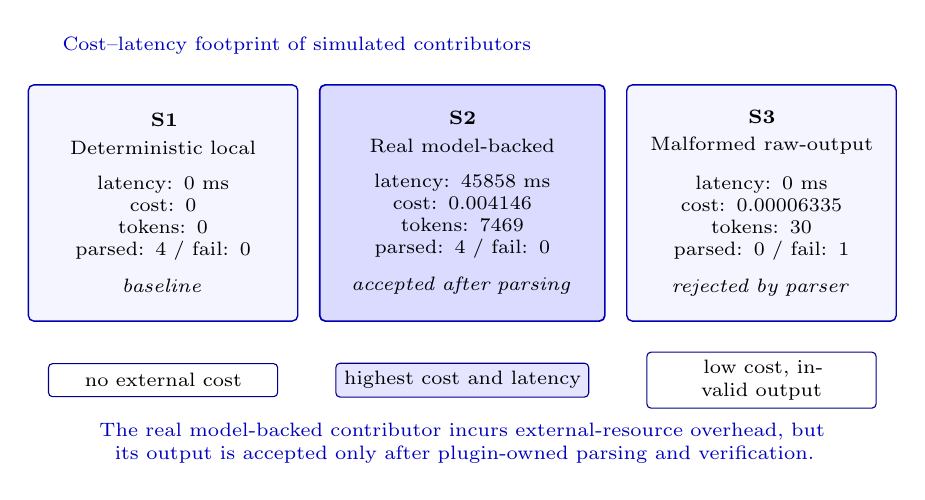
\begin{tikzpicture}[
  font=\scriptsize,
  card/.style={
    draw=blue!70!black,
    fill=blue!4,
    rounded corners=2pt,
    line width=0.5pt,
    align=center,
    inner sep=6pt
  },
  darkcard/.style={
    draw=blue!70!black,
    fill=blue!14,
    rounded corners=2pt,
    line width=0.6pt,
    align=center,
    inner sep=6pt
  },
  metric/.style={
    draw=blue!55!black,
    fill=white,
    rounded corners=1.5pt,
    line width=0.4pt,
    align=center,
    inner sep=3pt
  }
]

% Title
\node[
  font=\scriptsize,
  text=blue!75!black,
  anchor=west
] at (-5.2,3.0)
{Cost--latency footprint of simulated contributors};

% -------------------------------------------------------------------
% S1 card
% -------------------------------------------------------------------
\node[card, text width=3.0cm, minimum height=3.0cm] (s1) at (-3.8,1.0)
{
  \textbf{S1}\\[2pt]
  Deterministic local\\[6pt]

  \begin{tabular}{c}
  latency: 0 ms\\
  cost: 0\\
  tokens: 0\\
  parsed: 4 / fail: 0
  \end{tabular}\\[5pt]

  \textit{baseline}
};

% -------------------------------------------------------------------
% S2 card
% -------------------------------------------------------------------
\node[darkcard, text width=3.2cm, minimum height=3.0cm] (s2) at (0,1.0)
{
  \textbf{S2}\\[2pt]
  Real model-backed\\[6pt]

  \begin{tabular}{c}
  latency: 45858 ms\\
  cost: 0.004146\\
  tokens: 7469\\
  parsed: 4 / fail: 0
  \end{tabular}\\[5pt]

  \textit{accepted after parsing}
};

% -------------------------------------------------------------------
% S3 card
% -------------------------------------------------------------------
\node[card, text width=3.0cm, minimum height=3.0cm] (s3) at (3.8,1.0)
{
  \textbf{S3}\\[2pt]
  Malformed raw-output\\[6pt]

  \begin{tabular}{c}
  latency: 0 ms\\
  cost: 0.00006335\\
  tokens: 30\\
  parsed: 0 / fail: 1
  \end{tabular}\\[5pt]

  \textit{rejected by parser}
};

% Visual comparison strip
\node[
  metric,
  text width=2.7cm,
  minimum height=0.42cm
] at (-3.8,-1.25)
{no external cost};

\node[
  metric,
  fill=blue!10,
  text width=3.0cm,
  minimum height=0.42cm
] at (0,-1.25)
{highest cost and latency};

\node[
  metric,
  text width=2.7cm,
  minimum height=0.42cm
] at (3.8,-1.25)
{low cost, invalid output};

% Bottom explanation
\node[
  font=\scriptsize,
  text=blue!75!black,
  align=center,
  text width=10.6cm
] at (0,-2.05)
{The real model-backed contributor incurs external-resource overhead,
but its output is accepted only after plugin-owned parsing and verification.};

\end{tikzpicture}
}
}
\caption{\textcolor{blue}{Cost--latency footprint of simulated contributor profiles. The model-backed contributor increases cost and latency, while the malformed contributor remains cheap but produces no accepted parsed output.}}
\label{fig:cost-latency-footprint}
\end{figure}

Relative to the deterministic local profile, the real model-backed profile shows
no loss of task correctness, parser reliability, or retry behavior. Both profiles
complete the task correctly, both produce four parsed outputs, both record zero
parse failures, and the model-backed run requires no extra retry:
\[
  \begin{aligned}
    \mathrm{correct}_{\text{local}} &= \mathrm{correct}_{\text{model}} = 1,\\
    \mathrm{parsed}_{\text{local}} &= \mathrm{parsed}_{\text{model}} = 4,\\
    \mathrm{failures}_{\text{local}} &= \mathrm{failures}_{\text{model}} = 0,\\
    \Delta_{\mathrm{retry}} &= 0.
  \end{aligned}
\]
The real model-backed path introduces external-resource overhead in the explicit
\texttt{--real-transport} AI profile run reported in
\texttt{outputs/experiments/ai\_profile\_real}:
\[
  \Delta_{\mathrm{cost}}=0.004146,\qquad
  \Delta_{\mathrm{latency}}=45858\ \mathrm{ms}.
\]
{\color{blue}
This simulation supports the token-sharing interpretation of the protocol: contributors may differ in execution medium, reliability, and cost, but their outputs are mediated by a common parser, verifier, artifact, and accounting interface. Real model tokens can be shared into the task, yet they become useful only after the same evidence boundary as local compute.
}

\FloatBarrier

\subsection{Audit Footprint}
\label{subsec:audit-footprint}

{\color{blue}
The default suite records 1215 events and 510 artifacts. This footprint is not only execution telemetry; it is the evidence trail that lets TokenShare distinguish spent capacity from accepted contribution. A contribution economy without provenance collapses into trust in final answers. TokenShare instead keeps the intermediate requests, submissions, parser outcomes, verification reports, canonical bindings, merge records, and accounting facts inspectable.
}

\begin{figure}[!htbp]
\centering
{\color{blue}
\begin{tikzpicture}[x=0.0085cm,y=0.0042cm]
  \node[tslabel, anchor=west] at (0,1330) {Cumulative audit footprint};

  % axes
  \draw[tsline] (0,0) -- (1300,0);
  \draw[tsline] (0,0) -- (0,1250);

  \foreach \y/\lab in {0/0,400/400,800/800,1200/1200} {
    \draw[blue!15] (0,\y) -- (1250,\y);
    \node[tssmall, anchor=east] at (-30,\y) {\lab};
  }

  \foreach \x/\lab in {300/Exp.1,600/Exp.2,900/Exp.3,1200/Exp.4} {
    \draw[tsline] (\x,15) -- (\x,-15);
    \node[tssmall, anchor=north] at (\x,-40) {\lab};
  }

  % cumulative events
  \draw[blue!70!black, line width=0.9pt]
    (300,362) -- (600,842) -- (900,1027) -- (1200,1215);
  \foreach \x/\y in {300/362,600/842,900/1027,1200/1215}{
    \filldraw[draw=blue!70!black, fill=blue!35] (\x,\y) circle (3pt);
  }

  % cumulative artifacts
  \draw[blue!40!black, line width=0.9pt, dashed]
    (300,147) -- (600,337) -- (900,412) -- (1200,510);
  \foreach \x/\y in {300/147,600/337,900/412,1200/510}{
    \filldraw[draw=blue!40!black, fill=blue!8] (\x,\y) rectangle +(6,6);
  }

  \node[tssmall, anchor=west] at (850,1110) {cumulative events};
  \node[tssmall, anchor=west] at (850,455) {cumulative artifacts};
\end{tikzpicture}
}
\caption{\textcolor{blue}{Cumulative audit footprint across Experiments~1--4. The monotone increase reflects accumulated replay and artifact evidence, not merely final-answer records.}}
\label{fig:cumulative-audit-footprint}
\end{figure}

\begin{table}[!htbp]
\centering
\caption{\textcolor{blue}{Event and artifact footprint by experiment group.}}
\label{tab:audit-footprint}
\small
{\color{blue}
\begin{tabularx}{0.86\linewidth}{X>{\centering\arraybackslash}p{0.11\linewidth}>{\centering\arraybackslash}p{0.11\linewidth}>{\centering\arraybackslash}p{0.13\linewidth}>{\centering\arraybackslash}p{0.13\linewidth}}
\toprule
Group & Runs & Passed & Events & Artifacts \\
\midrule
Experiment 1 & 4 & 4 & 362 & 147 \\
Experiment 2 & 5 & 5 & 480 & 190 \\
Experiment 3 & 5 & 0 & 185 & 75 \\
Experiment 4 & 3 & 3 & 188 & 98 \\
\midrule
Total & 17 & 12 & 1215 & 510 \\
\bottomrule
\end{tabularx}
}
\end{table}

\FloatBarrier

\subsection{Limitations}
\label{subsec:limitations}

{\color{blue}
The results provide prototype-scale evidence for the TokenShare concept rather than a large-scale performance benchmark. The factorization tasks are fixed small integers, the default deterministic suite uses one seed, and the contributor-heterogeneity simulation uses a small number of executor profiles rather than a large population of real users. Accordingly, the evidence supports the conceptual claims that tokenized capacity can be decomposed into useful units, failed contributions can be isolated, key sharing mechanisms are necessary, and the lifecycle can cross task domains. Broader throughput scaling, stronger adversarial workloads, richer replay tooling, and multi-provider cost optimization remain separate evaluation targets.
}

\subsection{Summary}
\label{subsec:experiment-summary}

{\color{blue}
The experiments support four concept-level conclusions. First, TokenShare can convert shared bounded compute into a complete verified result. Second, invalid or malformed expenditure can remain auditable without becoming contribution. Third, parser ownership, verification, requeue, merge gating, and slot integrity are necessary for useful sharing. Fourth, the same contribution lifecycle supports factorization and real Lean proof production. The auxiliary contributor simulation further shows how local compute, real model tokens, and malformed output can enter one system while only verified evidence becomes accepted contribution.
}

% Restore the original caption behavior and text color after this section.
\makeatletter
\let\@makecaption\TSoldmakecaption
\makeatother
\endgroup
\normalcolor



\section{Related Work}

\paragraph{Distributed task allocation and market coordination.}
{\color{blue}
TokenShare builds on a long line of work on allocating work among distributed agents. The Contract Net Protocol introduced a negotiation pattern in which tasks are announced, potential contractors bid, and managers award work to selected agents \citep{smith1980contract}. Multi-robot task allocation later formalized the relation among agents, tasks, utilities, costs, and assignment structure \citep{gerkey2004formal}, while market-based coordination studied how decentralized bidding mechanisms can trade off communication cost, robustness, and solution quality \citep{dias2006market}. These works justify treating executor selection, leases, and retry as protocol-visible allocation decisions. TokenShare differs in that the allocated object is not a single atomic job: it is a recursively expandable task tree or DAG whose leaves may require model calls, local tools, external checkers, or bounded compute, and whose contribution records become eligible only after parser, verifier, canonical-selection, and merge boundaries succeed.
}

\paragraph{Complex crowdsourcing and decentralized crowdsourcing.}
{\color{blue}
Human-computation systems show that complex work can be decomposed, distributed, reviewed, and recomposed. CrowdForge proposes partition, map, and reduce primitives for crowdsourcing complex work \citep{kittur2011crowdforge}, and Turkomatic explores recursive task and workflow design for Mechanical Turk-style settings \citep{kulkarni2011turkomatic}. Blockchain-based crowdsourcing systems such as CrowdBC and decentralized HIT protocols study payment, dispute handling, and reduced reliance on centralized platforms \citep{li2018crowdbc,liang2022decentralizedhit}. For TokenShare, the relevant lesson is that decomposition and review need durable protocol evidence. The prototype generalizes this lesson to heterogeneous intelligent work by making plugin schemas, artifact references, verification reports, canonical choices, and merge policies part of a reusable local protocol substrate rather than a fixed human-task workflow.
}

\paragraph{Volunteer and distributed execution systems.}
{\color{blue}
Volunteer and cluster-computing systems provide practical lessons for unreliable and heterogeneous execution. BOINC supports volunteer scientific computation over devices that differ in capability, availability, and reliability \citep{anderson2020boinc}. MapReduce popularized partitioned data processing with automatic scheduling, failure handling, and re-execution on commodity clusters \citep{dean2004mapreduce}. Ray supports dynamic task graphs for AI applications \citep{moritz2018ray}, while Sparrow studies decentralized low-latency scheduling for short parallel tasks \citep{ousterhout2013sparrow}. TokenShare adopts the engineering vocabulary of leases, heartbeats, re-execution, and reassignment, but applies it to semantic and verifiable intelligent production: a work unit must include an input schema, output schema, verifier, provenance record, and merge rule.
}

\paragraph{Blockchains, verifiable computation, and useful work.}
{\color{blue}
Bitcoin demonstrates that mutually untrusted participants can be coordinated through a public ledger and proof-of-work incentives \citep{nakamoto2008bitcoin}. Ethereum generalizes the ledger into programmable smart contracts for decentralized applications \citep{buterin2014ethereum}. TrueBit studies interactive verification for expensive off-chain computation \citep{teutsch2019truebit}. Proof-of-useful-work systems such as Ofelimos attempt to replace artificial hash puzzles with useful optimization work \citep{fitzi2022ofelimos}. This literature informs TokenShare's use of public commitments, verifiable evidence, and replayable state transitions. The prototype brings that evidence discipline into a local useful-work setting: append-only events, content-addressed artifacts, verification reports, and deterministic replay are used to study task lifecycles across plugins and executors.
}

\paragraph{LLM decomposition, tool use, and multi-agent workflows.}
{\color{blue}
Recent LLM research shows that complex reasoning benefits from explicit intermediate structure. Decomposed Prompting, Least-to-Most Prompting, Tree of Thoughts, and ReAct all externalize decomposition, search, tool use, or intermediate reasoning states \citep{khot2023decomposed,zhou2023least,yao2023tree,yao2023react}. HuggingGPT and related tool-use systems use an LLM to plan subtasks and route them to external models or tools \citep{shen2023hugginggpt}. Multi-agent frameworks such as CAMEL, AutoGen, MetaGPT, and ChatDev further introduce role specialization, agent communication, and structured software-production workflows \citep{li2023camel,wu2023autogen,hong2024metagpt,qian2023chatdev}. These works motivate TokenShare's use of decomposition, roles, and tool-facing agents. TokenShare complements them by making allocation, parser boundaries, verification reports, canonical selection, merge, and contribution provenance explicit protocol objects rather than hidden orchestration state.
}

\paragraph{Verification-heavy intelligent tasks.}
Formal proof assistants provide a useful testbed because accepted outputs can be checked deterministically. The Lean mathematical library shows how a large community can maintain formalized mathematics in Lean \citep{mathlib2020}. miniF2F provides a cross-system benchmark for formal olympiad-level mathematics \citep{zheng2021minif2f}, and LeanDojo exposes Lean proof states, premises, interaction data, and benchmarks for retrieval-augmented theorem proving \citep{yang2023leandojo}. These works support our Lean proof-production application: TokenShare can treat a theorem, subgoal, tactic patch, error log, or auxiliary lemma as a task unit, while Lean supplies a replayable verifier.

\paragraph{Annotation quality and low-resource public-good NLP.}
Crowdsourced annotation research provides mature models for noisy contributors and uncertain labels. Dawid--Skene style aggregation estimates latent labels and worker error rates \citep{dawid1979maximum}; GLAD models both annotator ability and item difficulty \citep{whitehill2009glad}; MACE estimates annotator competence under noisy or adversarial conditions \citep{hovy2013mace}; and Snorkel shows how weak supervision sources can be combined into probabilistic labels \citep{ratner2017snorkel}. Low-resource language work also warns that public-good NLP is not merely a data-scarcity problem: language technologies are unevenly distributed across the world's languages \citep{joshi2020state}, participatory projects such as Masakhane emphasize community involvement \citep{nekoto2020participatory}, and NLLB combines large-scale data construction with human-centered evaluation for many languages \citep{nllb2022}. These lines motivate TokenShare's emphasis on provenance, uncertainty, expert escalation, and community review rather than treating generated artifacts as automatically authoritative.





\begin{table}[t]
\centering
\small
\caption{Positioning of TokenShare relative to adjacent work.}
\label{tab:related_positioning}
\begin{tabularx}{\linewidth}{p{0.22\linewidth} X X}
\toprule
Line of work & Main contribution & Gap addressed by TokenShare \\
\midrule
Task allocation & Negotiated or market-based assignment among agents & \textcolor{blue}{Recursive task DAGs with verification-aware routing and contribution eligibility} \\
Complex crowdsourcing & Human workflow decomposition and recomposition & Heterogeneous LLM, tool, compute, and human contributors with typed verifiers \\
Distributed execution & Scheduling and recovery for unreliable machines & Semantic intelligent work units with provenance, audit, and merge rules \\
\textcolor{blue}{Ledgered verification} & \textcolor{blue}{Public commitments, verifiable evidence, and replayable state transitions} & \textcolor{blue}{Event-sourced evidence and replayable contribution accounting for useful-work lifecycles} \\
LLM-agent systems & Planning, tool use, role specialization, and agent communication & \textcolor{blue}{Fault tolerance, parser and verifier boundaries, contribution attribution, and protocol-level evidence} \\
\bottomrule
\end{tabularx}
\end{table}


\section{Conclusion}

{\color{blue}
This paper presented TokenShare as a way to think about shared intelligent capacity. The central claim is that model tokens, tool calls, local compute, checker time, and human attention become useful at scale only when they can be decomposed into task units, bounded by requests, preserved as evidence, verified, merged, and counted as contributions.

The prototype uses distributed-systems mechanisms to make this concept concrete. Task DAGs create shareable units; leases and attempts bind resource expenditure to task identity; artifacts preserve evidence; plugins decide what counts as valid work; canonical selection and merge convert accepted evidence into parent progress; accounting records explain why a contribution counted. These mechanisms are not the end goal of TokenShare, but they are what make the concept credible.

The experiments provide initial evidence for the concept. Factorization shows that shared bounded compute can produce a verified result; failure injection shows that bad expenditure need not pollute accepted state; ablation shows which boundaries are necessary; Lean proof production shows that the lifecycle is not tied to one domain; and the AI contributor simulation shows how real model tokens can enter the system without bypassing parser and verifier authority. The scope of the evidence is deliberately prototype-scale: it establishes the contribution lifecycle and its necessary boundaries, while leaving benchmark breadth, contributor diversity, and resource-aware policy optimization outside the claims of this paper.
}


\section*{Ethical considerations}

{\color{blue}
The current experiments use arithmetic and formal-proof fixtures, but broader motivating domains such as annotation, knowledge organization, and low-resource language work can involve sensitive data, community knowledge, cultural context, and identity. Extending TokenShare to those settings requires licensing review, community consent, careful data governance, expert validation, minimal disclosure, and source-specific access control. Replayable provenance should support accountability while preserving uncertainty flags and avoiding overclaiming model-generated artifacts as community-authoritative without appropriate review.
}



\bibliographystyle{plainnat}
\bibliography{reference}

\end{document}
